\documentclass[conference]{IEEEtran}
\IEEEoverridecommandlockouts
% The preceding line is only needed to identify funding in the first footnote. If that is unneeded, please comment it out.
\usepackage{cite}
\usepackage{amsmath,amssymb,amsfonts}
\usepackage{algorithmic}
\usepackage{graphicx}
\usepackage{textcomp}
\usepackage{xcolor}
\def\BibTeX{{\rm B\kern-.05em{\sc i\kern-.025em b}\kern-.08em
    T\kern-.1667em\lower.7ex\hbox{E}\kern-.125emX}}
\begin{document}

\title{Classification of Hand Movements from sEMG Signals}

\author{\IEEEauthorblockN{Adithya Shastry}
\IEEEauthorblockA{\textit{Biomedical Engineering} \\
\textit{Columbia University}\\
New York, United States \\
ams2590@columbia.edu}
\and
\IEEEauthorblockN{Neil Kennedy }
\IEEEauthorblockA{\textit{Biomedical Engineering} \\
\textit{Columbia University}\\
New York, United States\\
nmk2142@columbia.edu}
\and
\IEEEauthorblockN{ Shahad Albrahim}
\IEEEauthorblockA{\textit{Biomedical Engineering} \\
\textit{Columbia University}\\
New York, United States \\
sha2139@columbia.edu}
}

\maketitle

\begin{abstract}
Advances in prosthetics and deep learning has allowed for the possibility of prosthetic limbs controlled by nervous signals. In this paper, we attempt to use a convolutional neural network and ResNet based Temporal Convolutional Network to achieve high accuracy of hand gesture classification from EMG data. These networks are useful in modelling time signal data in order to better classify different gestures. The models are trained on surface EMG data from the putEMG dataset, consisting of 24 channels of EMG data as participants performed 9 different hand signals. 
\end{abstract}



\section{Introduction}
In the field of biomechatronics, many different methods have been used to allow a human to control a prosthetic limb or an exoskeleton seamlessly. Traditional prosthetic limbs, and ones generally available to the public, are almost exclusively mechanically powered and actuated. This traditional approach has been known to be very uncomfortable, not intuitive, does not provide natural use of the limb, among many other issues \cite{b3}. To address this issue, many researchers and companies have developed solutions to use computerized control to create more complex and dynamic systems that can better resemble human anatomy and make the transition to using the prosthetic limb easier. However the biggest issue in this area is the ability of electrical and computer controlled systems to interface with the human body in such a way where the prosthetic limb simulates a real biological limb in as accurate a way as possible. In this paper we aim to experiment with various deep learning architectures to see which is best suited to analyse EMG gesture data from the putEMG data set.

\subsection{Prior work}
%Look through some of the research previously done and explain their findings
%TODO: Also look at the paper in the google drive
As a result of the impact that advancements in EMG data processing can have, as explained above, many researchers have employed various techniques such as traditional feature extraction based on the fundamentals of the EMG signal and human biology, usage of traditional machine learning and statistical techniques, as well as deep learning techniques. One group was able to achieve a 90\% accuracy using the support vector machine (SVM) traditional machine learning model after some feature extraction techniques were used on the raw data to better prime it for the SVM \cite{b1}. Another team was able process EMG data to classify gestures by using spiking neural networks (SNNs) that more closely model biological neurons as compared to artificial neural networks \cite{b4}. With this method of analysing EMG signals, the team was able to accomplish the same accuracy of gesture classification, but with 30 times the efficiency of traditional deep learning models. 

\subsection{Problem Statement}
In all of these previous works, the researching teams did not consider the temporal dimension of the EMG signal. Consideration, and accurate prediction of gesture, could drastically decrease the latency between a patient's muscular impulses of the patient and the expected outcome of the prosthetic limb. This decreased latency will have immense impacts on the usability of a prosthetic limb. As mentioned earlier, we will be investigating the effectiveness of various deep learning architectures in analyzing and classifying hand gestures.
\section{Materials and Methods}
\subsubsection{Data set and pre-processing}
The putEMG data set consists of 24 channels of sEMG data and a possibility of 9 hand gestures. There were multiple experimental procedures that the team had their subjects complete, however the sequential gesture data set was chosen. This sequential gesture data set consists of a sequence of 9 gestures which were sequentially held by the subject for 1 or 3 seconds. This sequence of gestures was then repeated a total of seven times \cite{b5}. As the subject was following the procedure of the experiment, sEMG signals from the 24 electrodes were continuously collected. Overall, the data set consisted of over 300 million data points for us to analyse. However, given the compute power we had access to on google colab and kaggle, processing the entire data set was not possible. 

In order to pare down the data set as well as build in a temporal dimension into it, the following steps were taken. The data set was imported and a sliding window of 1000 entries (about 0.195s) in the temporal dimension was separated and stored as a single data point to be used in the deep learning models. Since labels were given at each time step, the most common label in the sliding window was added as the overall label for the data point (spanning 1000 entries, or about 0.195s). To account for the immense amount of data available in the putEMG data set, a sample of 4000 temporal data points (extracted as described) were randomly chosen while keeping in mind the overall balance between the number of data points per label to allow for equal training on all hand gestures.

\subsection{Models}
%TODO: Explain the model architectures that were used
Three models, namely CNN, TCN and LSTM were trained and tested using the putEMG data.
\begin{figure}
    \centering
    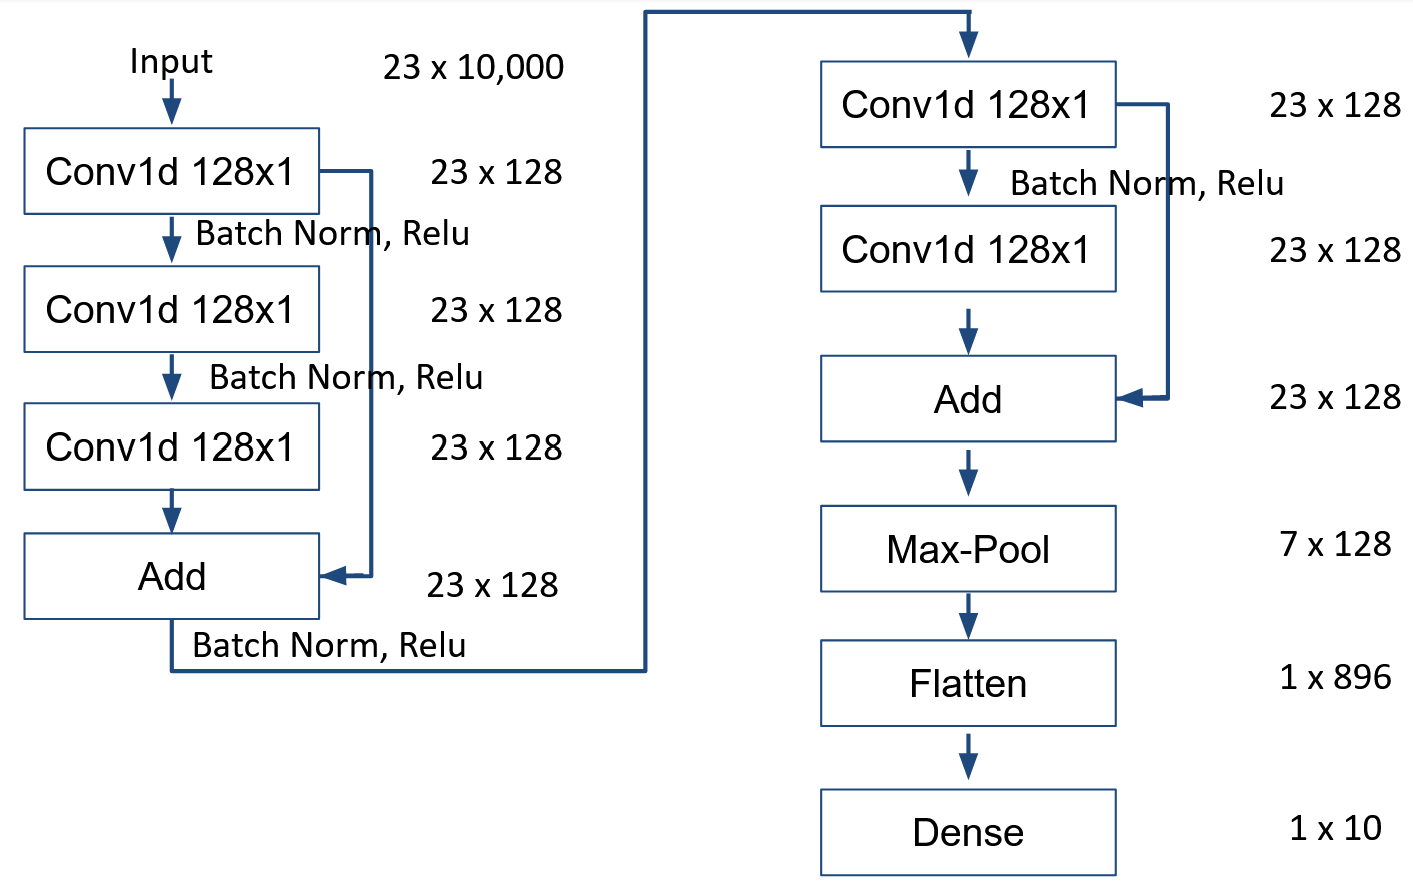
\includegraphics[scale = 0.55]{TCN.png}
    \caption{ Architecture for ResNet based TCN}
\end{figure}
The first model used was a ResNet based Temporal Convolutional Network (TCN). This model consisted of a series of convolutional layers and skip connections (Figure 1). The input is fed into a 1 dimension convolutional layer on each of the 23 channels before going through two residual blocks, then to a max-pool, flattening, and dense layer. Each of the residual blocks consist of two sets of a batch normalization layer, ReLU Activation layer, and convolutional layer, followed by a layer to combine the skip connection from before the residual block.\newline 
The convolutional layers used here are useful in extracting features from the short-term fluctuations in the signal. Therefore, there was a total of 5 convolutional layers in this model. In order to increase the receptive fields of nodes, dilation factors of 2 and 3 were used in the residual blocks, respectively. This allows the nodes to capture information from further back in time. The max-pool, flattening, and fully connected layers at the end allow the network to output a 1x10 vector, which is the shape of the labels after one-hot encoding. \newline
The best model was trained using an Adam optimizer, categorical crossentropy loss function, and learning rate of .001. It was run for 100 epochs with a batch size of 32, and the accuracy and loss were visualized (Figure 2).

Next, the CNN model was designed. The input shape to the CNN was set to (23, 10000). The first layer is the 1D convolution with 128 filters and a kernel size of 1. As it is a common choice for the number of filters to be between 32 and 512, we iterated through the following 32, 64, 128 and 256 and 128 filters produced the best accuracy. As for the kernel size, 1x1and 3x3 were tested for the highest accuracy which was achieved using the smallest kernel size. Next, a batch normalization was added to avoid over fitting and make the learning more efficient. After that, a 1D max pooling layer was added (to match the 1D convolution layer) with a pool size and stride of 2 which obtains an output shape of (None, 11, 128). This was followed by a flatten layer to lower the dimensionality to match the desired length of the training output data at the last layer. Then two hidden (dense) layers were added with the same activation function; Relu which is considered a default or common choice as a hidden layer activation function. However, the first hidden layer has 64 output units as opposed to 32 units for the second layer. Finally, the output layer has a softmax activation function that is essential for multinomial classification and 10 output units based on the expected number of classes. Following the designing stage, the model was compiled with “Adam” as the optimizer, “accuracy” as the validation metrics and since we one hot encoded the output training data, the loss function is set to categorical crossentropy instead of sparse categorical crossentropy.

For the training stage, we chose an epoch of 20 with early stopping from the keras library to prevent overfitting. The model was then evaluated through its accuracy, loss and the plotted confusion matrix where the latter is obtained from the available library called mlxtend. 


An LSTM model was also built and trained on the data, but had poor performance (accuracy $<40\%$) and therefore is not shown in the results section. Further work is needed to modify the LSTM to potentially achieve an accuracy similar to the TCN and CNN models. 

\section{Results}

The ResNet based TCN model was trained with various parameters and hyperparameters, including convolutional filter size, dilation, learning rate, and batch size. The model with the highest accuracy described in figure 1 was able to achieve an accuracy of 84.9\%. After 30 epochs, the loss increased in the validation set and parameters became overfit, therefore the model was saved and tested on the test set after 30 epochs (Figure 2). The predictions were visualized in a heatmap which showed that the model favored prediction of class 0, which corresponded to the flat hand position. 


\begin{figure}
    \centering
    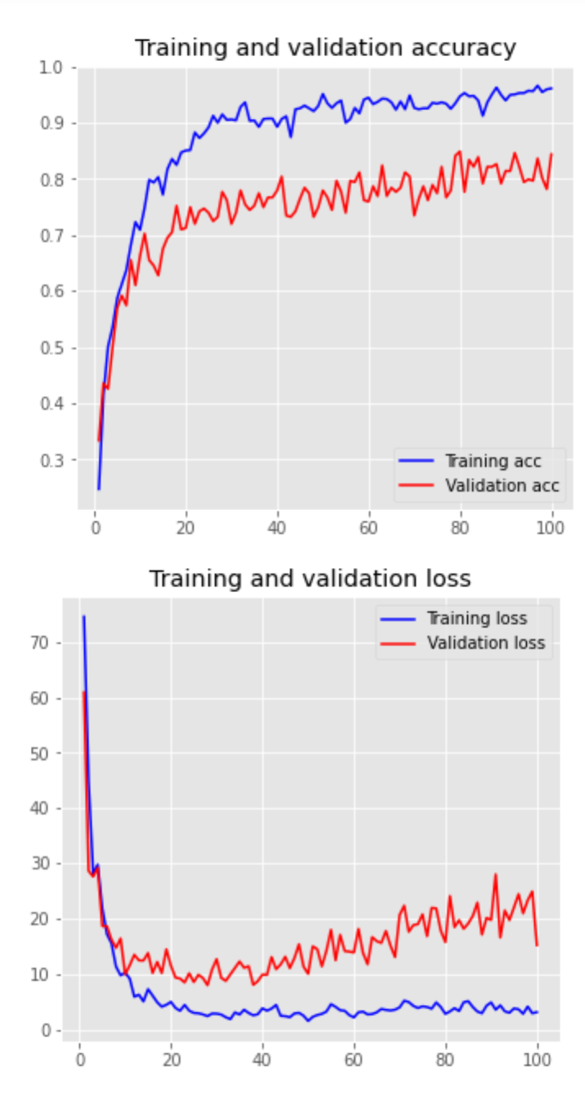
\includegraphics[scale = 1.2]{accuracy.png}
    
    \caption{ Training Accuracy and Loss for ResNet based TCN}
\end{figure}

\begin{figure}
    \centering
    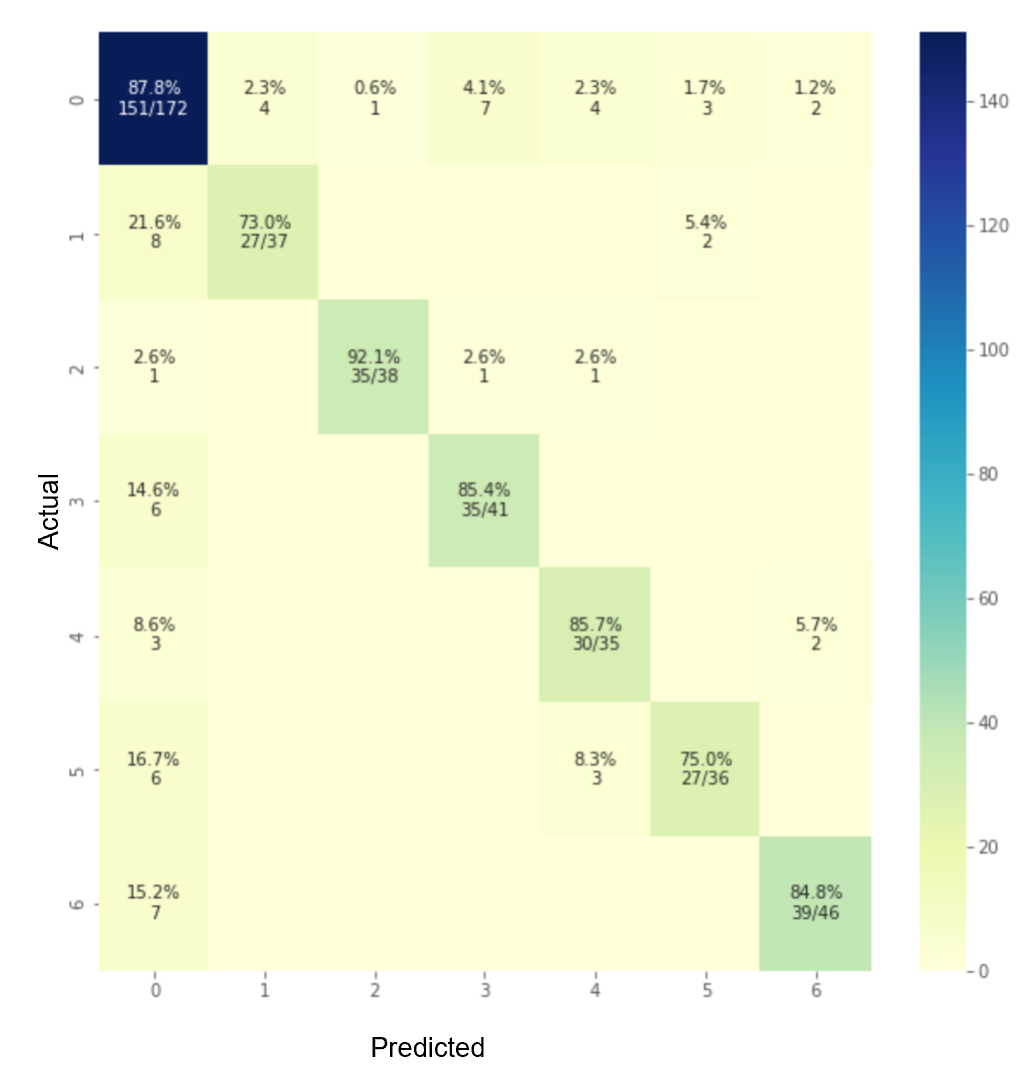
\includegraphics[scale = 0.7]{ResNetHeatmap.png}
    \caption{ Accuracy Heatmap for ResNet based TCN}
\end{figure}




The CNN model was first designed to have 3x3 kernel size and 64 filters. Due to limited computational capacity of PCs, the model was first trained using 1.6 percent of the total database as the original size is approximately 40 GBs.
The training was done using 20 epochs. This yielded a 62 percent accuracy. Then we increased the number of data used to roughly 4 percent and so did the accuracy which has increased to 82 percent which is almost 20 percent of the highest possible accuracy. To further raise the performance of the CNN model, different number of filters ( 32, 64, 128 and 256 ) and kernel sizes (1x1 and 3x3) were tested. All filters and kernel size combinations achieved similar accuracies ranging between 78 percent and 88 percent. However, a model with 128 filters and 1x1 kernel size raised the accuracy slightly to 92.5 percent. Figure 4 shows the latter model accuracy and loss over 20 epochs.


\begin{figure}
\centering
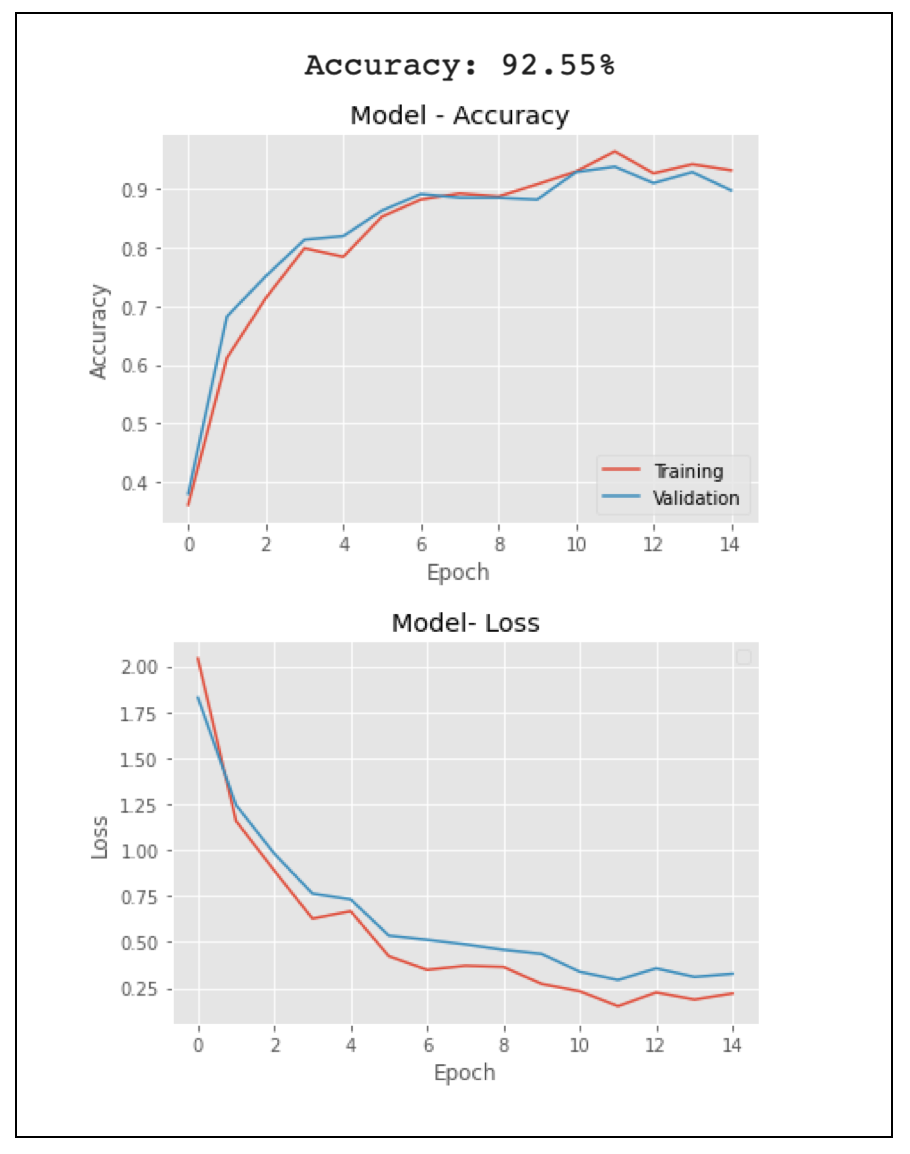
\includegraphics[scale = 0.55]{Acc_Loss.png}
\caption{the upper graph is the models accuracy plot against the number of epochs. The lower graph depicts the change in loss with increasing number of epochs. the accuracy of the CNN model is around 92.5 percent.}\end{figure}  It can be seen from the accuracy plot in figure 4 that there is a sharp increase in accuracy for epochs ranging from 0 to 10. Then it start reaching a plateau all the way to 20 epochs with an actual slight enhance in accuracy at 20 epochs. After 20 epochs, the accuracy stayed relatively the same so to help the model train faster while getting the best possible accuracy was set to 20 epochs. 
Next, the confusion matrix was plotted (Figure 6) to inspect how accurate the prediction was with regards to each class. The highest prediction was for class 0 which represent a fist with an accuracy of 99 percent followed by the 5th class (pinch thumb-ring hand gesture) with 97 percent accuracy and 2nd class (extension) with 0.95 percent accuracy. Table 1 summarizes hand gestures with corresponding prediction accuracies obtained from the confusion matrix.\newline
\begin{figure} 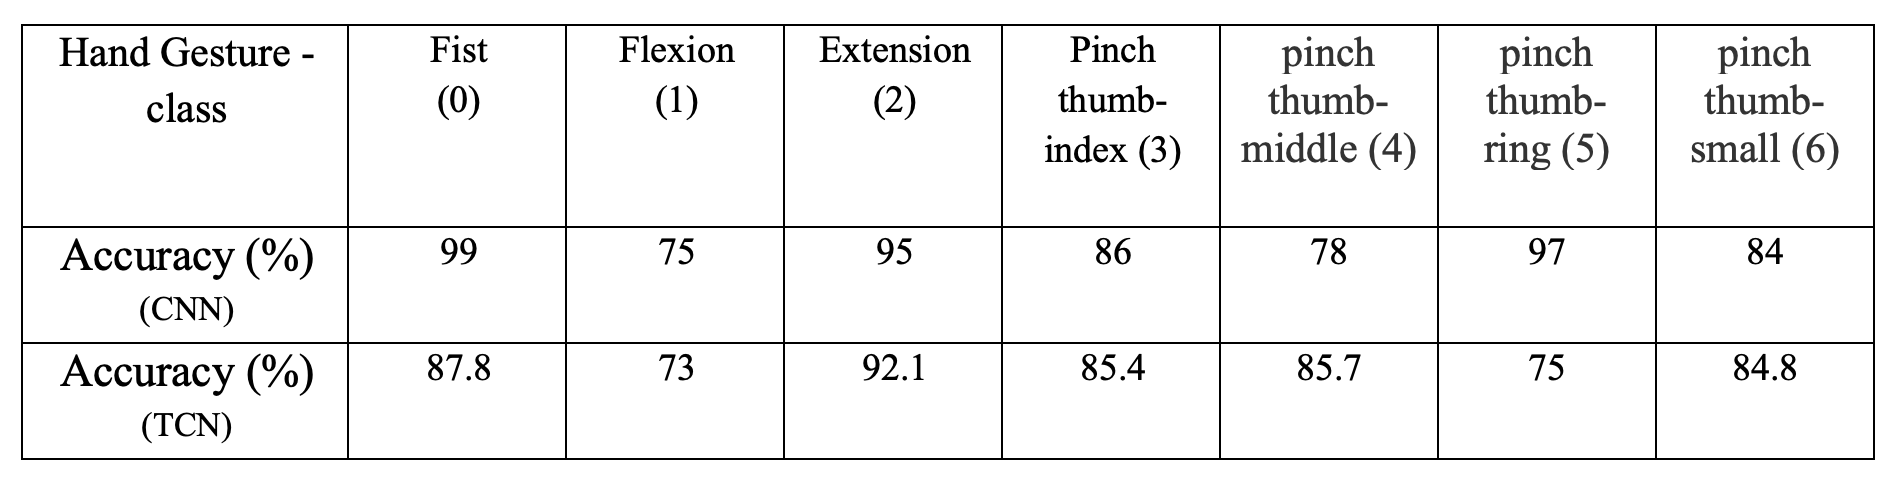
\includegraphics[scale = 0.27]{Table.png}
\centering
\caption{Table 1: hand gestures prediction by both the CNN \& TCN models with accuracies ranging from 73 percent to 99 percent}
\end{figure}

\begin{figure}
\centering
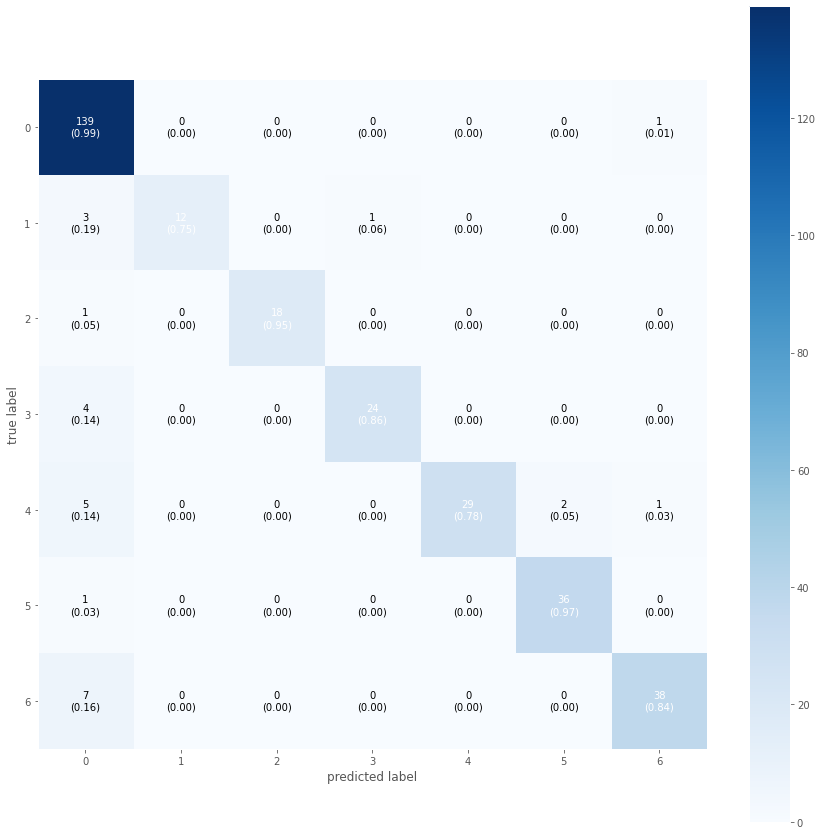
\includegraphics[scale = 0.3]{CM.png}
\caption{confusion matrix of the CNN model. The model performed best at predicting the outputs for class 0 while the worst was class 1}
\end{figure}
\newline




\section{Conclusion and Future Work}
This paper utilized two deep learning models - a ResNet based TCN and a CNN - to classify hand gesture data from the putEMG dataset. The CNN achieved an accuracy of 92.5\%, which outperformed the ResNet based TCN with an accuracy of 84.9\%. However, we only used a portion of the putEMG dataset due to computational limitations, so with more compute power we should be able to improve the results further. Considering the size of our dataset, our 92.5\% accuracy was fairly high for a seven class classification problem, and comparable to other studies. In addition to using the full dataset, future work is needed to further adjust parameters of these networks and maximize accuracy, as well as to improve the LSTM model to perform comparably to the other architectures. 

\begin{thebibliography}{00}
\bibitem{b1} Kaczmarek, Piotr, et al. “PutEMG—A Surface Electromyography Hand Gesture Recognition Dataset.” Sensors, vol. 19, no. 16, 2019, p. 3548., https://doi.org/10.3390/s19163548.
\bibitem{b3} Keszler, Mary. “What You Should Know before Getting a Prosthetic Leg.” Johns Hopkins Medicine, https://www.hopkinsmedicine.org/health/wellness-and-prevention/what-to-know-before-getting-prosthetic-leg. 
\bibitem{b4} Ceolini, Enea, et al. “Hand-Gesture Recognition Based on EMG and Event-Based Camera Sensor Fusion: A Benchmark in Neuromorphic Computing.” Frontiers in Neuroscience, vol. 14, 2020, https://doi.org/10.3389/fnins.2020.00637. 
\bibitem{b5} “PUTEMG: SEMG Gesture and Force Recognition Datasets.” Biomedical Engineering and Biocybernetics Team, https://biolab.put.poznan.pl/putemg-dataset/. 
\end{thebibliography}

\end{document}
